\documentclass{article}
\usepackage[utf8]{inputenc}
\usepackage[spanish]{babel}
\usepackage{listings}
\usepackage{subfigure}
\usepackage{graphicx}
\usepackage{url}
\usepackage{multirow}
\usepackage{multicol}
\usepackage{color}
\usepackage{booktabs}
\usepackage{float}
\usepackage{amsmath,amssymb,amscd,amsthm}
%\usepackage{verbatim}
\usepackage{hyperref}
\hypersetup{
    colorlinks=true,
    linkcolor=blue,
    filecolor=magenta,      
    urlcolor=cyan,
}
\usepackage[margin=3cm,twoside]{geometry} 
\setlength{\parindent}{0pt}
\setlength{\parskip}{1em}
\usepackage{fancyvrb}
\usepackage{enumerate}
\newcommand\ql{\textquotedblleft}
\newcommand\qr{\textquotedblright}


\newcommand\E{\ensuremath{\mathbb{E}}}
\newcommand\N{\ensuremath{\mathbb{N}}}
\renewcommand{\P}{\ensuremath{\mathbb{P}}}
\newcommand\Q{\ensuremath{\mathbb{Q}}}
\newcommand\R{\ensuremath{\mathbb{R}}}
\newcommand\Z{\ensuremath{\mathbb{Z}}}

\newcommand\Om{\ensuremath{\Omega}}
\newcommand{\w}{\ensuremath{\omega}}

\newcommand\var[1]{\, \mathrm{Var} \left( #1 \right)}

\newcommand\pr[1]{\, \mathbb{P} \left( #1 \right)}

\newcommand\cov[1]{\, \mathrm{Cov} \left( #1 \right)}

\newcommand\espe[1]{\, \mathbb{E} \lbrack #1 \rbrack}



\definecolor{mygreen}{rgb}{0,0.6,0}
\definecolor{mygray}{rgb}{0.5,0.5,0.5}
\definecolor{mymauve}{rgb}{0.58,0,0.82}
\lstset{ 
  backgroundcolor=\color{white},   % choose the background color; you must add \usepackage{color} or \usepackage{xcolor}; should come as last argument
  basicstyle=\footnotesize,        % the size of the fonts that are used for the code
  breakatwhitespace=false,         % sets if automatic breaks should only happen at whitespace
  breaklines=true,                 % sets automatic line breaking
  captionpos=b,                    % sets the caption-position to bottom
  commentstyle=\color{mygreen},    % comment style
  deletekeywords={...},            % if you want to delete keywords from the given language
  escapeinside={\%*}{)},          % if you want to add LaTeX within your code
  extendedchars=true,              % lets you use non-ASCII characters; for 8-bits encodings only, does not work with UTF-8
  firstnumber=1,                % start line enumeration with line 1000
  frame=single,	                   % adds a frame around the code
  keepspaces=true,                 % keeps spaces in text, useful for keeping indentation of code (possibly needs columns=flexible)
  keywordstyle=\color{blue},       % keyword style
  language=Octave,                 % the language of the code
  morekeywords={*,...},            % if you want to add more keywords to the set
  numbers=left,                    % where to put the line-numbers; possible values are (none, left, right)
  numbersep=5pt,                   % how far the line-numbers are from the code
  numberstyle=\tiny\color{mygray}, % the style that is used for the line-numbers
  rulecolor=\color{black},         % if not set, the frame-color may be changed on line-breaks within not-black text (e.g. comments (green here))
  showspaces=false,                % show spaces everywhere adding particular underscores; it overrides 'showstringspaces'
  showstringspaces=false,          % underline spaces within strings only
  showtabs=false,                  % show tabs within strings adding particular underscores
  stepnumber=1,                    % the step between two line-numbers. If it's 1, each line will be numbered
  stringstyle=\color{mymauve},     % string literal style
  tabsize=2,	                   % sets default tabsize to 2 spaces
  title=\lstname                  % show the filename of files included with \lstinputlisting; also try caption instead of title
}
\usepackage{etoolbox}
\makeatletter
\providecommand{\subtitle}[1]{% add subtitle to \maketitle
  \apptocmd{\@title}{\par {\large #1 \par}}{}{}
}
\RecustomVerbatimCommand{\VerbatimInput}{VerbatimInput}%
{fontsize=\footnotesize,
	%
	frame=lines,  % top and bottom rule only
	framesep=2em, % separation between frame and text
	rulecolor=\color{mygreen},
	%
	label=\fbox{\color{black} prueba.txt},
	labelposition=topline,
	%
	commandchars=\|\(\), % escape character and argument delimiters for
	% commands within the verbatim
	%commentchar=*        % comment character
}
\renewcommand{\theenumi}{\roman{enumi}}
\newtheorem{teor}{Teorema}
\makeatother
 \title{Tarea 13 de Modelos Probabilistas Aplicados}
\subtitle{Ley de los grandes números}
\author{5271}
\date{\today}

\begin{document}

\maketitle
\section{Introducción}
En este documento se presenta las nociones básicas sobre la ley de los grandes números, ejemplos y aplicaciones.
\section{Ley de los grandes números}
LA ley de los grandes números plantea formalmente que con una sucesión de variables aleatorias independientes e idénticamente distribuidas con varianza finita se asegura que el promedio de las n primeras observaciones (variables aleatorias) se acerca a la media teórica cuando el número n de repeticiones tiende hacia infinito. Lo anterior se apoya en el teorema 8.2 del libro ``\textit{Introduction to Probability}''\cite{libProba}:

Sean $X_1,X_2,...,X_n$ un proceso de pruebas independientes e igualmente distribuidos con un valor esperado finito $\mu = E[X]$ y una y una varianza finita $\sigma^2 = \mbox{Var}[X]$. Sea $S_n = X_1 + X_2 + \ldots + X_n$. Entonces para cualquier valor de $\epsilon > 0$ y n que tiende al infinito se tiene:
\begin{align}
  \lim_{n \rightarrow \infty} P\left( \left | \frac{S_n}{n} - \mu \right | \geq \epsilon \right )  & = 0  \\
  \lim_{n \rightarrow \infty} P\left( \left | \frac{S_n}{n} - \mu \right | < \epsilon \right ) &= 1
\end{align}
Un caso particular de esta ley es el principio de estabilidad de las frecuencias, o teorema de Bernoulli, que ya hemos visto. Efectivamente, recordemos que una variable de Bernoulli es aquella que toma solo el valor 0 o 1 cuando no ocurre (u ocurre, respectivamente) un suceso $A$   con probabilidades $1-p$ y $p$. Sumar $n$ variables de Bernoulli es contar el número de veces que se repite el suceso $A$ en $n$ pruebas. Una variable de Bernoulli tiene media $p$. Luego la media de $n$ medias sera también $p$.

 Para una mejor comprensión de lo anteriormente expuesto se tomará como ejemplo la resolución del ejercicio 3 de la página 312 del mismo libro, que dice:
 
\textit{Write a program to toss a coin 10,000 times. Let $S_n$ be the number of heads in the first $n$ tosses. Have your program print out, after every 1000 tosses, $S_n - \frac{n}{2}$. On the basis of this simulation, is it correct to say that you can expect heads about half of the time when you toss a coin a large number of times?} 

Para resolver este ejercicio se realiza el programa \ref{cod:1} en lenguaje R \cite{R} que se muestra a continuación.

\begin{center}
\lstinputlisting[ language=R, firstline=1, lastline=12]{Tarea13.R}
\label{cod:1}
\end{center}
 El cuadro \ref{tab:1} de la página \pageref{tab:1} se puede observar claramente, que para el programa \ref{cod:1} donde se ejecuta diez simulaciones de 1000 lanzamientos de una moneda donde la cara vale uno y la cruz 0. Es correcto decir que puede esperar cara la mitad de las veces cuando lanza una moneda una gran cantidad de veces. En la figura \ref{fig:1} de la página \pageref{fig:1} se muestra los resultados para 100 repeticiones.

\begin{table}[H]
  \centering
  \caption{Resultados de la simulación de sacar cara en el lanzamiento de una moneda}
  \vspace{0.1cm}
    \begin{tabular}{rrr}
    \toprule
          & \multicolumn{1}{c}{\textit{\textbf{n}}} & \multicolumn{1}{c}{\textit{\textbf{Sn}}} \\
    \midrule
    1     & 1,000 & 0.513 \\
    2     & 2,000 & 0.511 \\
    3     & 3,000 & 0.510 \\
    4     & 4,000 & 0.506 \\
    5     & 5,000 & 0.504 \\
    6     & 6,000 & 0.505 \\
    7     & 7,000 & 0.503 \\
    8     & 8,000 & 0.502 \\
    9     & 9,000 & 0.502 \\
    10    & 10,000 & 0.502 \\
    \bottomrule
    \end{tabular}%
  \label{tab:1}%
\end{table}%
\begin{figure}
    \centering
    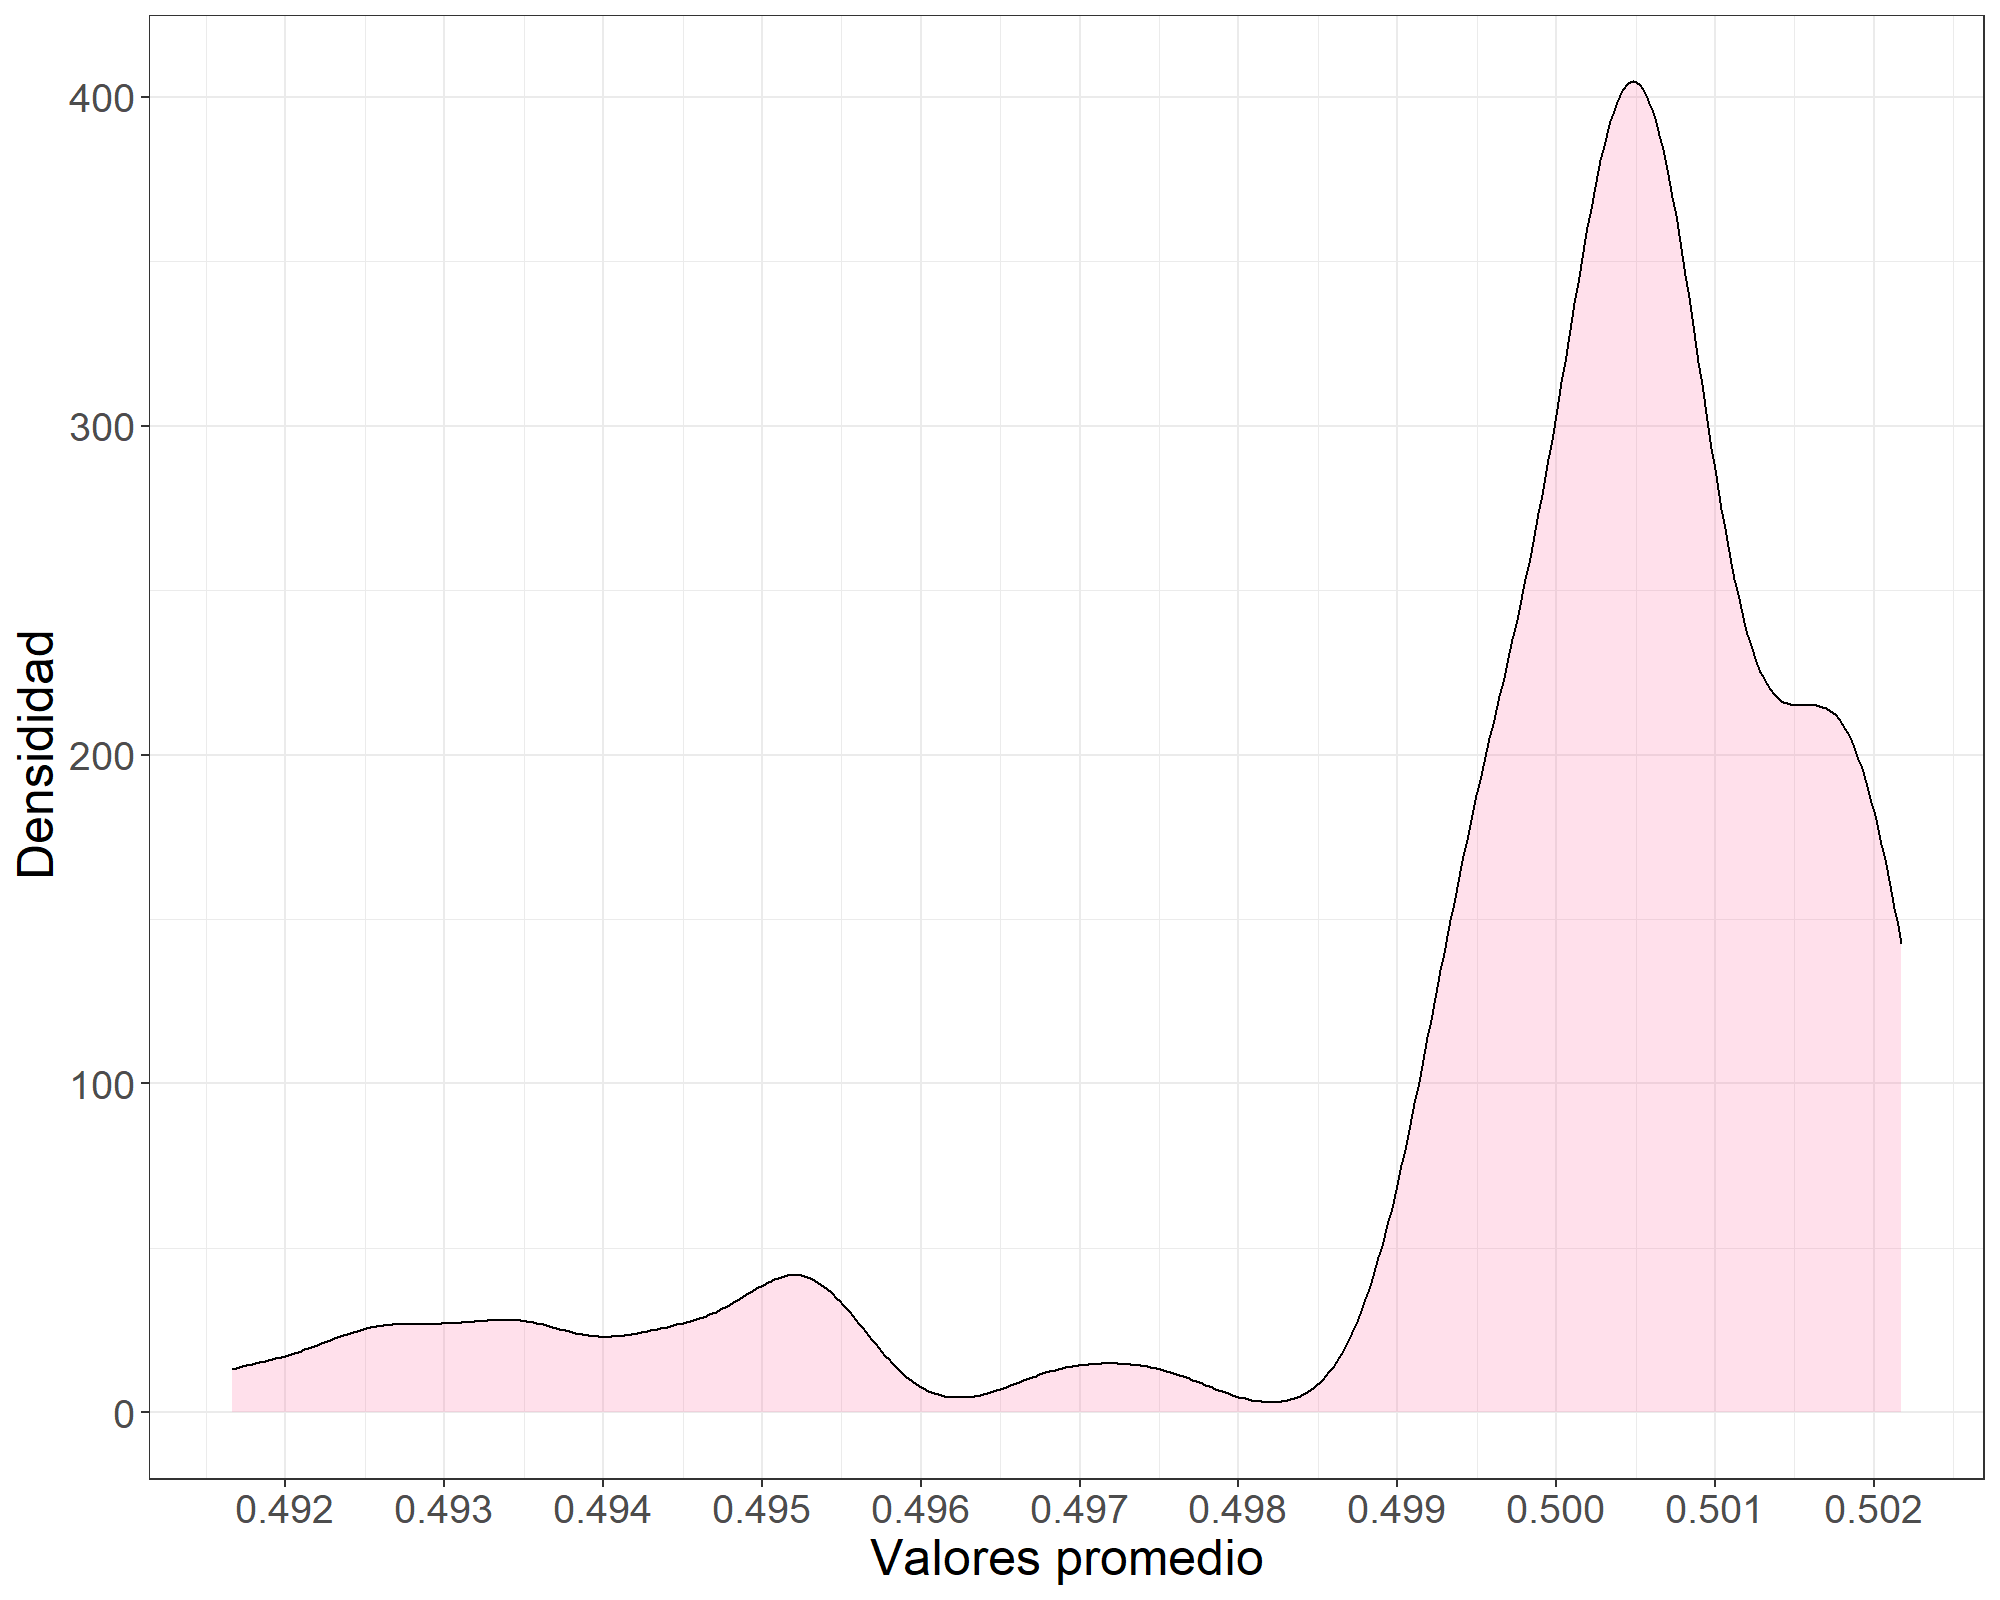
\includegraphics[scale=0.35]{figuras/ejercicio13.png}
    \caption{Diagrama de densidad de los resultados para 100 repeticiones del experimento.}
    \label{fig:1}
\end{figure}
\section{Aplicación en la estimación de subconjuntos en un método estocástico de ramificación y poda } 
 En \cite{norkin1998branch}, se propone un método estocástico de ramificación y poda para resolver problemas de optimización global estocástica. Como en el caso determinista, el conjunto factible se divide en subconjuntos compactos. Para guiar el proceso de partición, el método utiliza estimaciones estocásticas superior e inferior del valor óptimo de la función objetivo en cada subconjunto. Y se demuestra la convergencia del método y se obtienen estimaciones de precisión aleatorias. Se discuten los métodos para construir límites estocásticos superior e inferior a través de la ley de los grandes números. Las consideraciones teóricas la ilustran con un ejemplo de un problema de ubicación de instalaciones.
 
En el método estocástico de ramificación y poda \cite{norkin1998branch} se construye una secuencia de conjuntos $X^{k}(\omega) \subset X^{k-1}(\omega)$, y se tiene que estimar el valor de cota inferior $L(\cdot)$ en el límite que establece $X^{\ast} =\lim_k X(\omega)$, usando observaciones independientes de variables aleatorias $\epsilon (X^k)$ tales que $\espe{\epsilon (X^k)}=L(X^{k})$. A tal efecto, en\cite{norkin1998branch} se utiliza la siguiente estimación:
\begin{equation}
    L_k(X^k)= \frac{1}{k}\sum_{s=1}^[k] \to L(X^{\ast}).
\end{equation}
\newpage
\bibliographystyle{plain}
\bibliography{Biblio}

\end{document}

